\section{Attributes Class Reference}
\label{classAttributes}\index{Attributes@{Attributes}}
{\tt \#include $<$attributes.h$>$}

Inheritance diagram for Attributes::\begin{figure}[H]
\begin{center}
\leavevmode
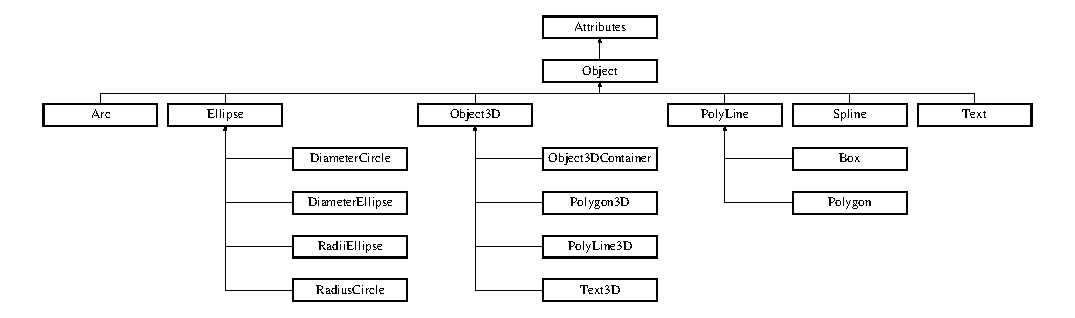
\includegraphics[height=3.82812cm]{classAttributes}
\end{center}
\end{figure}
\subsection*{Public Types}
\begin{CompactItemize}
\item 
enum {\bf Line\-Styles} \{ {\bf Default\-Line\-Style} =  -1, 
{\bf Solid} =  0, 
{\bf Dashed} =  1, 
{\bf Dotted} =  2, 
{\bf Dash\-Dotted} =  3, 
{\bf Dash\-Double\-Dotted} =  4, 
{\bf Dash\-Triple\-Dotted} =  5
 \}
\item 
enum {\bf Colors} \{ {\bf Default\-Color} =  -1, 
{\bf Black} =  0, 
{\bf Blue} =  1, 
{\bf Green} =  2, 
{\bf Cyan} =  3, 
{\bf Red} =  4, 
{\bf Magenta} =  5, 
{\bf Yellow} =  6, 
{\bf White} =  7, 
{\bf Gold} =  31
 \}
\item 
enum {\bf Fonts} \{ {\bf Default\-Latex} =  0, 
{\bf Roman} =  1, 
{\bf Bold} =  2, 
{\bf Italic} =  3, 
{\bf Sans\-Serif} =  4, 
{\bf Type\-Writer} =  5, 
{\bf Default\-Post\-Script} =  -1, 
{\bf Times\-Roman} =  0, 
{\bf Times\-Italic} =  1, 
{\bf Times\-Bold} =  2, 
{\bf Times\-Bold\-Italic} =  3, 
{\bf Avant\-Garde\-Book} =  4, 
{\bf Avant\-Garde\-Book\-Oblique} =  5, 
{\bf Avant\-Garde\-Demi} =  6, 
{\bf Avant\-Garde\-Demi\-Oblique} =  7, 
{\bf Bookman\-Light} =  8, 
{\bf Bookman\-Light\-Italic} =  9, 
{\bf Bookman\-Demi} =  10, 
{\bf Bookman\-Demi\-Italic} =  11, 
{\bf Courier} =  12, 
{\bf Courier\-Oblique} =  13, 
{\bf Courier\-Bold} =  14, 
{\bf Courier\-Bold\-Oblique} =  15, 
{\bf Helvetica} =  16, 
{\bf Helvetica\-Oblique} =  17, 
{\bf Helvetica\-Bold} =  18, 
{\bf Helvetica\-Bold\-Oblique} =  19, 
{\bf Helvetica\-Narrow} =  20, 
{\bf Helvetica\-Narrow\-Oblique} =  21, 
{\bf Helvetica\-Narrow\-Bold} =  22, 
{\bf Helvetica\-Narrow\-Bold\-Oblique} =  23, 
{\bf New\-Century\-Schoolbook\-Roman} =  24, 
{\bf New\-Century\-Schoolbook\-Italic} =  25, 
{\bf New\-Century\-Schoolbook\-Bold} =  26, 
{\bf New\-Century\-Schoolbook\-Bold\-Italic} =  27, 
{\bf Palatino\-Roman} =  28, 
{\bf Palatino\-Italic} =  29, 
{\bf Palatino\-Bold} =  30, 
{\bf Palatino\-Bold\-Italic} =  31, 
{\bf Symbol} =  32, 
{\bf Zapf\-Chancery\-Medium\-Italic} =  32, 
{\bf Zapf\-Dingbats} =  34
 \}
\item 
enum {\bf Font\-Flags} \{ {\bf Rigid} =  1, 
{\bf Latex} =  2, 
{\bf Rigid\-Latex} =  3, 
{\bf Post\-Script} =  4, 
{\bf Rigid\-Post\-Script} =  5, 
{\bf Latex\-Post\-Script} =  6, 
{\bf Rigid\-Latex\-Post\-Script} =  7, 
{\bf Hidden} =  8, 
{\bf Rigid\-Hidden} =  9, 
{\bf Latex\-Hidden} =  10, 
{\bf Rigid\-Latex\-Hidden} =  11, 
{\bf Post\-Script\-Hidden} =  12, 
{\bf Rigid\-Post\-Script\-Hidden} =  13, 
{\bf Latex\-Post\-Script\-Hidden} =  14, 
{\bf Rigid\-Latex\-Post\-Script\-Hidden} =  15
 \}
\end{CompactItemize}
\subsection*{Public Methods}
\begin{CompactItemize}
\item 
{\bf Attributes} ()
\item 
{\bf $\sim$Attributes} ()
\item 
void {\bf set\-Line\-Style} ({\bf Line\-Styles} {\bf line\-Style})
\item 
void {\bf set\-Thickness} (int {\bf thickness})
\item 
void {\bf set\-Pen\-Color} ({\bf Colors} {\bf pen\-Color})
\item 
void {\bf set\-Fill\-Color} ({\bf Colors} {\bf fill\-Color})
\item 
void {\bf set\-Depth} (int {\bf depth})
\item 
void {\bf set\-Pen\-Style} (int {\bf pen\-Style})
\item 
void {\bf set\-Area\-Fill} (int {\bf area\-Fill})
\item 
void {\bf set\-Style\-Val} (float {\bf style\-Val})
\item 
void {\bf set\-Join\-Style} (int {\bf join\-Style})
\item 
void {\bf set\-Cap\-Style} (int {\bf cap\-Style})
\item 
void {\bf set\-Radius} (int {\bf radius})
\item 
void {\bf set\-Forward\-Arrow\-Bool} (int {\bf forward\-Arrow\-Bool})
\item 
void {\bf set\-Backward\-Arrow\-Bool} (int {\bf backward\-Arrow\-Bool})
\item 
void {\bf set\-Forward\-Arrow} ({\bf Arrow} {\bf forward\-Arrow})
\item 
void {\bf set\-Backward\-Arrow} ({\bf Arrow} {\bf backward\-Arrow})
\item 
void {\bf set\-Angle} (float {\bf angle})
\item 
void {\bf set\-Font} ({\bf Fonts} {\bf font})
\item 
void {\bf set\-Font\-Size} (float {\bf font\-Size})
\item 
void {\bf set\-Font\-Flags} ({\bf Font\-Flags} {\bf font\-Flags})
\item 
void {\bf set\-Height} (float {\bf height})
\item 
void {\bf set\-Length} (float {\bf length})
\item 
void {\bf set\-Attributes} (Attributes attributes)
\item 
{\bf Line\-Styles} {\bf get\-Line\-Style} ()
\item 
int {\bf get\-Thickness} ()
\item 
{\bf Colors} {\bf get\-Pen\-Color} ()
\item 
{\bf Colors} {\bf get\-Fill\-Color} ()
\item 
int {\bf get\-Depth} ()
\item 
int {\bf get\-Pen\-Style} ()
\item 
int {\bf get\-Area\-Fill} ()
\item 
float {\bf get\-Style\-Val} ()
\item 
int {\bf get\-Join\-Style} ()
\item 
int {\bf get\-Cap\-Style} ()
\item 
int {\bf get\-Radius} ()
\item 
int {\bf get\-Forward\-Arrow\-Bool} ()
\item 
int {\bf get\-Backward\-Arrow\-Bool} ()
\item 
{\bf Arrow} {\bf get\-Forward\-Arrow} ()
\item 
{\bf Arrow} {\bf get\-Backward\-Arrow} ()
\item 
float {\bf get\-Angle} ()
\item 
{\bf Fonts} {\bf get\-Font} ()
\item 
float {\bf get\-Font\-Size} ()
\item 
{\bf Font\-Flags} {\bf get\-Font\-Flags} ()
\item 
float {\bf get\-Height} ()
\item 
float {\bf get\-Length} ()
\item 
Attributes {\bf get\-Attributes} ()
\end{CompactItemize}
\subsection*{Protected Attributes}
\begin{CompactItemize}
\item 
{\bf Line\-Styles} {\bf line\-Style}
\item 
int {\bf thickness}
\item 
{\bf Colors} {\bf pen\-Color}
\item 
{\bf Colors} {\bf fill\-Color}
\item 
int {\bf depth}
\item 
int {\bf pen\-Style}
\item 
int {\bf area\-Fill}
\item 
float {\bf style\-Val}
\item 
int {\bf join\-Style}
\item 
int {\bf cap\-Style}
\item 
int {\bf radius}
\item 
int {\bf forward\-Arrow\-Bool}
\item 
int {\bf backward\-Arrow\-Bool}
\item 
float {\bf angle}
\item 
{\bf Fonts} {\bf font}
\item 
float {\bf font\-Size}
\item 
{\bf Font\-Flags} {\bf font\-Flags}
\item 
float {\bf height}
\item 
float {\bf length}
\item 
{\bf Arrow} {\bf forward\-Arrow}
\item 
{\bf Arrow} {\bf backward\-Arrow}
\end{CompactItemize}


\subsection{Detailed Description}
Generic class to handle the attributes of objects. \begin{Desc}
\item[Author: ]\par
Anthony Liekens \end{Desc}




\subsection{Member Enumeration Documentation}
\index{Attributes@{Attributes}!Colors@{Colors}}
\index{Colors@{Colors}!Attributes@{Attributes}}
\subsubsection{\setlength{\rightskip}{0pt plus 5cm}enum Attributes::Colors}\label{classAttributes_s75}


\begin{Desc}
\item[Enumeration values: ]\par
\begin{description}
\index{DefaultColor@{DefaultColor}!Attributes@{Attributes}}\index{Attributes@{Attributes}!DefaultColor@{DefaultColor}}\item[{\em 
{\em Default\-Color}\label{classAttributes_s75s7}
}]\index{Black@{Black}!Attributes@{Attributes}}\index{Attributes@{Attributes}!Black@{Black}}\item[{\em 
{\em Black}\label{classAttributes_s75s8}
}]\index{Blue@{Blue}!Attributes@{Attributes}}\index{Attributes@{Attributes}!Blue@{Blue}}\item[{\em 
{\em Blue}\label{classAttributes_s75s9}
}]\index{Green@{Green}!Attributes@{Attributes}}\index{Attributes@{Attributes}!Green@{Green}}\item[{\em 
{\em Green}\label{classAttributes_s75s10}
}]\index{Cyan@{Cyan}!Attributes@{Attributes}}\index{Attributes@{Attributes}!Cyan@{Cyan}}\item[{\em 
{\em Cyan}\label{classAttributes_s75s11}
}]\index{Red@{Red}!Attributes@{Attributes}}\index{Attributes@{Attributes}!Red@{Red}}\item[{\em 
{\em Red}\label{classAttributes_s75s12}
}]\index{Magenta@{Magenta}!Attributes@{Attributes}}\index{Attributes@{Attributes}!Magenta@{Magenta}}\item[{\em 
{\em Magenta}\label{classAttributes_s75s13}
}]\index{Yellow@{Yellow}!Attributes@{Attributes}}\index{Attributes@{Attributes}!Yellow@{Yellow}}\item[{\em 
{\em Yellow}\label{classAttributes_s75s14}
}]\index{White@{White}!Attributes@{Attributes}}\index{Attributes@{Attributes}!White@{White}}\item[{\em 
{\em White}\label{classAttributes_s75s15}
}]\index{Gold@{Gold}!Attributes@{Attributes}}\index{Attributes@{Attributes}!Gold@{Gold}}\item[{\em 
{\em Gold}\label{classAttributes_s75s16}
}]\end{description}
\end{Desc}

\index{Attributes@{Attributes}!FontFlags@{FontFlags}}
\index{FontFlags@{FontFlags}!Attributes@{Attributes}}
\subsubsection{\setlength{\rightskip}{0pt plus 5cm}enum Attributes::Font\-Flags}\label{classAttributes_s77}


\begin{Desc}
\item[Enumeration values: ]\par
\begin{description}
\index{Rigid@{Rigid}!Attributes@{Attributes}}\index{Attributes@{Attributes}!Rigid@{Rigid}}\item[{\em 
{\em Rigid}\label{classAttributes_s77s59}
}]\index{Latex@{Latex}!Attributes@{Attributes}}\index{Attributes@{Attributes}!Latex@{Latex}}\item[{\em 
{\em Latex}\label{classAttributes_s77s60}
}]\index{RigidLatex@{RigidLatex}!Attributes@{Attributes}}\index{Attributes@{Attributes}!RigidLatex@{RigidLatex}}\item[{\em 
{\em Rigid\-Latex}\label{classAttributes_s77s61}
}]\index{PostScript@{PostScript}!Attributes@{Attributes}}\index{Attributes@{Attributes}!PostScript@{PostScript}}\item[{\em 
{\em Post\-Script}\label{classAttributes_s77s62}
}]\index{RigidPostScript@{RigidPostScript}!Attributes@{Attributes}}\index{Attributes@{Attributes}!RigidPostScript@{RigidPostScript}}\item[{\em 
{\em Rigid\-Post\-Script}\label{classAttributes_s77s63}
}]\index{LatexPostScript@{LatexPostScript}!Attributes@{Attributes}}\index{Attributes@{Attributes}!LatexPostScript@{LatexPostScript}}\item[{\em 
{\em Latex\-Post\-Script}\label{classAttributes_s77s64}
}]\index{RigidLatexPostScript@{RigidLatexPostScript}!Attributes@{Attributes}}\index{Attributes@{Attributes}!RigidLatexPostScript@{RigidLatexPostScript}}\item[{\em 
{\em Rigid\-Latex\-Post\-Script}\label{classAttributes_s77s65}
}]\index{Hidden@{Hidden}!Attributes@{Attributes}}\index{Attributes@{Attributes}!Hidden@{Hidden}}\item[{\em 
{\em Hidden}\label{classAttributes_s77s66}
}]\index{RigidHidden@{RigidHidden}!Attributes@{Attributes}}\index{Attributes@{Attributes}!RigidHidden@{RigidHidden}}\item[{\em 
{\em Rigid\-Hidden}\label{classAttributes_s77s67}
}]\index{LatexHidden@{LatexHidden}!Attributes@{Attributes}}\index{Attributes@{Attributes}!LatexHidden@{LatexHidden}}\item[{\em 
{\em Latex\-Hidden}\label{classAttributes_s77s68}
}]\index{RigidLatexHidden@{RigidLatexHidden}!Attributes@{Attributes}}\index{Attributes@{Attributes}!RigidLatexHidden@{RigidLatexHidden}}\item[{\em 
{\em Rigid\-Latex\-Hidden}\label{classAttributes_s77s69}
}]\index{PostScriptHidden@{PostScriptHidden}!Attributes@{Attributes}}\index{Attributes@{Attributes}!PostScriptHidden@{PostScriptHidden}}\item[{\em 
{\em Post\-Script\-Hidden}\label{classAttributes_s77s70}
}]\index{RigidPostScriptHidden@{RigidPostScriptHidden}!Attributes@{Attributes}}\index{Attributes@{Attributes}!RigidPostScriptHidden@{RigidPostScriptHidden}}\item[{\em 
{\em Rigid\-Post\-Script\-Hidden}\label{classAttributes_s77s71}
}]\index{LatexPostScriptHidden@{LatexPostScriptHidden}!Attributes@{Attributes}}\index{Attributes@{Attributes}!LatexPostScriptHidden@{LatexPostScriptHidden}}\item[{\em 
{\em Latex\-Post\-Script\-Hidden}\label{classAttributes_s77s72}
}]\index{RigidLatexPostScriptHidden@{RigidLatexPostScriptHidden}!Attributes@{Attributes}}\index{Attributes@{Attributes}!RigidLatexPostScriptHidden@{RigidLatexPostScriptHidden}}\item[{\em 
{\em Rigid\-Latex\-Post\-Script\-Hidden}\label{classAttributes_s77s73}
}]\end{description}
\end{Desc}

\index{Attributes@{Attributes}!Fonts@{Fonts}}
\index{Fonts@{Fonts}!Attributes@{Attributes}}
\subsubsection{\setlength{\rightskip}{0pt plus 5cm}enum Attributes::Fonts}\label{classAttributes_s76}


Enumeration of font faces. The following fonts can be used to set the font face of an object : \{$\backslash$tt Default\-Latex, Roman, Bold, Italic, Sans\-Serif, Type\-Writer, Default\-Post\-Script, Times\-Roman, Times\-Italic, Times\-Bold, Times\-Bold\-Italic, Avant\-Garde\-Book, Avant\-Garde\-Book\-Oblique, Avant\-Garde\-Demi, Avant\-Garde\-Demi\-Oblique, Bookman\-Light, Bookman\-Light\-Italic, Bookman\-Demi, Bookman\-Demi\-Italic, Courier, Courier\-Oblique, Courier\-Bold, Courier\-Bold\-Oblique, Helvetica, Helvetica\-Oblique, Helvetica\-Bold, Helvetica\-Bold\-Oblique, Helvetica\-Narrow, Helvetica\-Narrow\-Oblique, Helvetica\-Narrow\-Bold, Helvetica\-Narrow\-Bold\-Oblique, New\-Century\-Schoolbook\-Roman, New\-Century\-Schoolbook\-Italic, New\-Century\-Schoolbook\-Bold, New\-Century\-Schoolbook\-Bold\-Italic, Palatino\-Roman, Palatino\-Italic, Palatino\-Bold, Palatino\-Bold\-Italic, Symbol, Zapf\-Chancery\-Medium\-Italic, Zapf\-Dingbats\} \begin{Desc}
\item[Enumeration values: ]\par
\begin{description}
\index{DefaultLatex@{DefaultLatex}!Attributes@{Attributes}}\index{Attributes@{Attributes}!DefaultLatex@{DefaultLatex}}\item[{\em 
{\em Default\-Latex}\label{classAttributes_s76s17}
}]\index{Roman@{Roman}!Attributes@{Attributes}}\index{Attributes@{Attributes}!Roman@{Roman}}\item[{\em 
{\em Roman}\label{classAttributes_s76s18}
}]\index{Bold@{Bold}!Attributes@{Attributes}}\index{Attributes@{Attributes}!Bold@{Bold}}\item[{\em 
{\em Bold}\label{classAttributes_s76s19}
}]\index{Italic@{Italic}!Attributes@{Attributes}}\index{Attributes@{Attributes}!Italic@{Italic}}\item[{\em 
{\em Italic}\label{classAttributes_s76s20}
}]\index{SansSerif@{SansSerif}!Attributes@{Attributes}}\index{Attributes@{Attributes}!SansSerif@{SansSerif}}\item[{\em 
{\em Sans\-Serif}\label{classAttributes_s76s21}
}]\index{TypeWriter@{TypeWriter}!Attributes@{Attributes}}\index{Attributes@{Attributes}!TypeWriter@{TypeWriter}}\item[{\em 
{\em Type\-Writer}\label{classAttributes_s76s22}
}]\index{DefaultPostScript@{DefaultPostScript}!Attributes@{Attributes}}\index{Attributes@{Attributes}!DefaultPostScript@{DefaultPostScript}}\item[{\em 
{\em Default\-Post\-Script}\label{classAttributes_s76s23}
}]\index{TimesRoman@{TimesRoman}!Attributes@{Attributes}}\index{Attributes@{Attributes}!TimesRoman@{TimesRoman}}\item[{\em 
{\em Times\-Roman}\label{classAttributes_s76s24}
}]\index{TimesItalic@{TimesItalic}!Attributes@{Attributes}}\index{Attributes@{Attributes}!TimesItalic@{TimesItalic}}\item[{\em 
{\em Times\-Italic}\label{classAttributes_s76s25}
}]\index{TimesBold@{TimesBold}!Attributes@{Attributes}}\index{Attributes@{Attributes}!TimesBold@{TimesBold}}\item[{\em 
{\em Times\-Bold}\label{classAttributes_s76s26}
}]\index{TimesBoldItalic@{TimesBoldItalic}!Attributes@{Attributes}}\index{Attributes@{Attributes}!TimesBoldItalic@{TimesBoldItalic}}\item[{\em 
{\em Times\-Bold\-Italic}\label{classAttributes_s76s27}
}]\index{AvantGardeBook@{AvantGardeBook}!Attributes@{Attributes}}\index{Attributes@{Attributes}!AvantGardeBook@{AvantGardeBook}}\item[{\em 
{\em Avant\-Garde\-Book}\label{classAttributes_s76s28}
}]\index{AvantGardeBookOblique@{AvantGardeBookOblique}!Attributes@{Attributes}}\index{Attributes@{Attributes}!AvantGardeBookOblique@{AvantGardeBookOblique}}\item[{\em 
{\em Avant\-Garde\-Book\-Oblique}\label{classAttributes_s76s29}
}]\index{AvantGardeDemi@{AvantGardeDemi}!Attributes@{Attributes}}\index{Attributes@{Attributes}!AvantGardeDemi@{AvantGardeDemi}}\item[{\em 
{\em Avant\-Garde\-Demi}\label{classAttributes_s76s30}
}]\index{AvantGardeDemiOblique@{AvantGardeDemiOblique}!Attributes@{Attributes}}\index{Attributes@{Attributes}!AvantGardeDemiOblique@{AvantGardeDemiOblique}}\item[{\em 
{\em Avant\-Garde\-Demi\-Oblique}\label{classAttributes_s76s31}
}]\index{BookmanLight@{BookmanLight}!Attributes@{Attributes}}\index{Attributes@{Attributes}!BookmanLight@{BookmanLight}}\item[{\em 
{\em Bookman\-Light}\label{classAttributes_s76s32}
}]\index{BookmanLightItalic@{BookmanLightItalic}!Attributes@{Attributes}}\index{Attributes@{Attributes}!BookmanLightItalic@{BookmanLightItalic}}\item[{\em 
{\em Bookman\-Light\-Italic}\label{classAttributes_s76s33}
}]\index{BookmanDemi@{BookmanDemi}!Attributes@{Attributes}}\index{Attributes@{Attributes}!BookmanDemi@{BookmanDemi}}\item[{\em 
{\em Bookman\-Demi}\label{classAttributes_s76s34}
}]\index{BookmanDemiItalic@{BookmanDemiItalic}!Attributes@{Attributes}}\index{Attributes@{Attributes}!BookmanDemiItalic@{BookmanDemiItalic}}\item[{\em 
{\em Bookman\-Demi\-Italic}\label{classAttributes_s76s35}
}]\index{Courier@{Courier}!Attributes@{Attributes}}\index{Attributes@{Attributes}!Courier@{Courier}}\item[{\em 
{\em Courier}\label{classAttributes_s76s36}
}]\index{CourierOblique@{CourierOblique}!Attributes@{Attributes}}\index{Attributes@{Attributes}!CourierOblique@{CourierOblique}}\item[{\em 
{\em Courier\-Oblique}\label{classAttributes_s76s37}
}]\index{CourierBold@{CourierBold}!Attributes@{Attributes}}\index{Attributes@{Attributes}!CourierBold@{CourierBold}}\item[{\em 
{\em Courier\-Bold}\label{classAttributes_s76s38}
}]\index{CourierBoldOblique@{CourierBoldOblique}!Attributes@{Attributes}}\index{Attributes@{Attributes}!CourierBoldOblique@{CourierBoldOblique}}\item[{\em 
{\em Courier\-Bold\-Oblique}\label{classAttributes_s76s39}
}]\index{Helvetica@{Helvetica}!Attributes@{Attributes}}\index{Attributes@{Attributes}!Helvetica@{Helvetica}}\item[{\em 
{\em Helvetica}\label{classAttributes_s76s40}
}]\index{HelveticaOblique@{HelveticaOblique}!Attributes@{Attributes}}\index{Attributes@{Attributes}!HelveticaOblique@{HelveticaOblique}}\item[{\em 
{\em Helvetica\-Oblique}\label{classAttributes_s76s41}
}]\index{HelveticaBold@{HelveticaBold}!Attributes@{Attributes}}\index{Attributes@{Attributes}!HelveticaBold@{HelveticaBold}}\item[{\em 
{\em Helvetica\-Bold}\label{classAttributes_s76s42}
}]\index{HelveticaBoldOblique@{HelveticaBoldOblique}!Attributes@{Attributes}}\index{Attributes@{Attributes}!HelveticaBoldOblique@{HelveticaBoldOblique}}\item[{\em 
{\em Helvetica\-Bold\-Oblique}\label{classAttributes_s76s43}
}]\index{HelveticaNarrow@{HelveticaNarrow}!Attributes@{Attributes}}\index{Attributes@{Attributes}!HelveticaNarrow@{HelveticaNarrow}}\item[{\em 
{\em Helvetica\-Narrow}\label{classAttributes_s76s44}
}]\index{HelveticaNarrowOblique@{HelveticaNarrowOblique}!Attributes@{Attributes}}\index{Attributes@{Attributes}!HelveticaNarrowOblique@{HelveticaNarrowOblique}}\item[{\em 
{\em Helvetica\-Narrow\-Oblique}\label{classAttributes_s76s45}
}]\index{HelveticaNarrowBold@{HelveticaNarrowBold}!Attributes@{Attributes}}\index{Attributes@{Attributes}!HelveticaNarrowBold@{HelveticaNarrowBold}}\item[{\em 
{\em Helvetica\-Narrow\-Bold}\label{classAttributes_s76s46}
}]\index{HelveticaNarrowBoldOblique@{HelveticaNarrowBoldOblique}!Attributes@{Attributes}}\index{Attributes@{Attributes}!HelveticaNarrowBoldOblique@{HelveticaNarrowBoldOblique}}\item[{\em 
{\em Helvetica\-Narrow\-Bold\-Oblique}\label{classAttributes_s76s47}
}]\index{NewCenturySchoolbookRoman@{NewCenturySchoolbookRoman}!Attributes@{Attributes}}\index{Attributes@{Attributes}!NewCenturySchoolbookRoman@{NewCenturySchoolbookRoman}}\item[{\em 
{\em New\-Century\-Schoolbook\-Roman}\label{classAttributes_s76s48}
}]\index{NewCenturySchoolbookItalic@{NewCenturySchoolbookItalic}!Attributes@{Attributes}}\index{Attributes@{Attributes}!NewCenturySchoolbookItalic@{NewCenturySchoolbookItalic}}\item[{\em 
{\em New\-Century\-Schoolbook\-Italic}\label{classAttributes_s76s49}
}]\index{NewCenturySchoolbookBold@{NewCenturySchoolbookBold}!Attributes@{Attributes}}\index{Attributes@{Attributes}!NewCenturySchoolbookBold@{NewCenturySchoolbookBold}}\item[{\em 
{\em New\-Century\-Schoolbook\-Bold}\label{classAttributes_s76s50}
}]\index{NewCenturySchoolbookBoldItalic@{NewCenturySchoolbookBoldItalic}!Attributes@{Attributes}}\index{Attributes@{Attributes}!NewCenturySchoolbookBoldItalic@{NewCenturySchoolbookBoldItalic}}\item[{\em 
{\em New\-Century\-Schoolbook\-Bold\-Italic}\label{classAttributes_s76s51}
}]\index{PalatinoRoman@{PalatinoRoman}!Attributes@{Attributes}}\index{Attributes@{Attributes}!PalatinoRoman@{PalatinoRoman}}\item[{\em 
{\em Palatino\-Roman}\label{classAttributes_s76s52}
}]\index{PalatinoItalic@{PalatinoItalic}!Attributes@{Attributes}}\index{Attributes@{Attributes}!PalatinoItalic@{PalatinoItalic}}\item[{\em 
{\em Palatino\-Italic}\label{classAttributes_s76s53}
}]\index{PalatinoBold@{PalatinoBold}!Attributes@{Attributes}}\index{Attributes@{Attributes}!PalatinoBold@{PalatinoBold}}\item[{\em 
{\em Palatino\-Bold}\label{classAttributes_s76s54}
}]\index{PalatinoBoldItalic@{PalatinoBoldItalic}!Attributes@{Attributes}}\index{Attributes@{Attributes}!PalatinoBoldItalic@{PalatinoBoldItalic}}\item[{\em 
{\em Palatino\-Bold\-Italic}\label{classAttributes_s76s55}
}]\index{Symbol@{Symbol}!Attributes@{Attributes}}\index{Attributes@{Attributes}!Symbol@{Symbol}}\item[{\em 
{\em Symbol}\label{classAttributes_s76s56}
}]\index{ZapfChanceryMediumItalic@{ZapfChanceryMediumItalic}!Attributes@{Attributes}}\index{Attributes@{Attributes}!ZapfChanceryMediumItalic@{ZapfChanceryMediumItalic}}\item[{\em 
{\em Zapf\-Chancery\-Medium\-Italic}\label{classAttributes_s76s57}
}]\index{ZapfDingbats@{ZapfDingbats}!Attributes@{Attributes}}\index{Attributes@{Attributes}!ZapfDingbats@{ZapfDingbats}}\item[{\em 
{\em Zapf\-Dingbats}\label{classAttributes_s76s58}
}]\end{description}
\end{Desc}

\index{Attributes@{Attributes}!LineStyles@{LineStyles}}
\index{LineStyles@{LineStyles}!Attributes@{Attributes}}
\subsubsection{\setlength{\rightskip}{0pt plus 5cm}enum Attributes::Line\-Styles}\label{classAttributes_s74}


Enumeration of line styles. The following line styles can be used to set the line style of an object : \{$\backslash$tt Default\-Line\-Style, Solid, Dashed, Dotted, Dash\-Dotted, Dash\-Dotted, Dash\-Double\-Dotted, Dash\-Triple\-Dotted\} \begin{Desc}
\item[Enumeration values: ]\par
\begin{description}
\index{DefaultLineStyle@{DefaultLineStyle}!Attributes@{Attributes}}\index{Attributes@{Attributes}!DefaultLineStyle@{DefaultLineStyle}}\item[{\em 
{\em Default\-Line\-Style}\label{classAttributes_s74s0}
}]\index{Solid@{Solid}!Attributes@{Attributes}}\index{Attributes@{Attributes}!Solid@{Solid}}\item[{\em 
{\em Solid}\label{classAttributes_s74s1}
}]\index{Dashed@{Dashed}!Attributes@{Attributes}}\index{Attributes@{Attributes}!Dashed@{Dashed}}\item[{\em 
{\em Dashed}\label{classAttributes_s74s2}
}]\index{Dotted@{Dotted}!Attributes@{Attributes}}\index{Attributes@{Attributes}!Dotted@{Dotted}}\item[{\em 
{\em Dotted}\label{classAttributes_s74s3}
}]\index{DashDotted@{DashDotted}!Attributes@{Attributes}}\index{Attributes@{Attributes}!DashDotted@{DashDotted}}\item[{\em 
{\em Dash\-Dotted}\label{classAttributes_s74s4}
}]\index{DashDoubleDotted@{DashDoubleDotted}!Attributes@{Attributes}}\index{Attributes@{Attributes}!DashDoubleDotted@{DashDoubleDotted}}\item[{\em 
{\em Dash\-Double\-Dotted}\label{classAttributes_s74s5}
}]\index{DashTripleDotted@{DashTripleDotted}!Attributes@{Attributes}}\index{Attributes@{Attributes}!DashTripleDotted@{DashTripleDotted}}\item[{\em 
{\em Dash\-Triple\-Dotted}\label{classAttributes_s74s6}
}]\end{description}
\end{Desc}



\subsection{Constructor \& Destructor Documentation}
\index{Attributes@{Attributes}!Attributes@{Attributes}}
\index{Attributes@{Attributes}!Attributes@{Attributes}}
\subsubsection{\setlength{\rightskip}{0pt plus 5cm}Attributes::Attributes ()}\label{classAttributes_a0}


Constructor. Sets default values for all attributes. \index{Attributes@{Attributes}!~Attributes@{$\sim$Attributes}}
\index{~Attributes@{$\sim$Attributes}!Attributes@{Attributes}}
\subsubsection{\setlength{\rightskip}{0pt plus 5cm}Attributes::$\sim$Attributes ()}\label{classAttributes_a1}


Destructor. 

\subsection{Member Function Documentation}
\index{Attributes@{Attributes}!getAngle@{getAngle}}
\index{getAngle@{getAngle}!Attributes@{Attributes}}
\subsubsection{\setlength{\rightskip}{0pt plus 5cm}float Attributes::get\-Angle ()\hspace{0.3cm}{\tt  [inline]}}\label{classAttributes_a39}


Returns the angle. \begin{Desc}
\item[Returns: ]\par
float \end{Desc}


Reimplemented in {\bf Ellipse} {\rm (p.\,\pageref{classEllipse_a4})}.\index{Attributes@{Attributes}!getAreaFill@{getAreaFill}}
\index{getAreaFill@{getAreaFill}!Attributes@{Attributes}}
\subsubsection{\setlength{\rightskip}{0pt plus 5cm}int Attributes::get\-Area\-Fill ()\hspace{0.3cm}{\tt  [inline]}}\label{classAttributes_a30}


Returns the area fill. \begin{Desc}
\item[Returns: ]\par
int \end{Desc}
\index{Attributes@{Attributes}!getAttributes@{getAttributes}}
\index{getAttributes@{getAttributes}!Attributes@{Attributes}}
\subsubsection{\setlength{\rightskip}{0pt plus 5cm}Attributes Attributes::get\-Attributes ()\hspace{0.3cm}{\tt  [inline]}}\label{classAttributes_a45}


Returns itself. This method can be used to extract attributes out of {\bf Object} {\rm (p.\,\pageref{classObject})} instances. \begin{Desc}
\item[Returns: ]\par
Instance of Attributes \end{Desc}
\index{Attributes@{Attributes}!getBackwardArrow@{getBackwardArrow}}
\index{getBackwardArrow@{getBackwardArrow}!Attributes@{Attributes}}
\subsubsection{\setlength{\rightskip}{0pt plus 5cm}{\bf Arrow} Attributes::get\-Backward\-Arrow ()\hspace{0.3cm}{\tt  [inline]}}\label{classAttributes_a38}


Returns the backward arrow. \begin{Desc}
\item[Returns: ]\par
Instance of {\bf Arrow} {\rm (p.\,\pageref{classArrow})} \end{Desc}
\index{Attributes@{Attributes}!getBackwardArrowBool@{getBackwardArrowBool}}
\index{getBackwardArrowBool@{getBackwardArrowBool}!Attributes@{Attributes}}
\subsubsection{\setlength{\rightskip}{0pt plus 5cm}int Attributes::get\-Backward\-Arrow\-Bool ()\hspace{0.3cm}{\tt  [inline]}}\label{classAttributes_a36}


Returns the backward arrow bool value (0 = do not draw an arrow, 1 = draw an arrow). \begin{Desc}
\item[Returns: ]\par
int \end{Desc}
\index{Attributes@{Attributes}!getCapStyle@{getCapStyle}}
\index{getCapStyle@{getCapStyle}!Attributes@{Attributes}}
\subsubsection{\setlength{\rightskip}{0pt plus 5cm}int Attributes::get\-Cap\-Style ()\hspace{0.3cm}{\tt  [inline]}}\label{classAttributes_a33}


Returns the cap style. \begin{Desc}
\item[Returns: ]\par
int \end{Desc}
\index{Attributes@{Attributes}!getDepth@{getDepth}}
\index{getDepth@{getDepth}!Attributes@{Attributes}}
\subsubsection{\setlength{\rightskip}{0pt plus 5cm}int Attributes::get\-Depth ()\hspace{0.3cm}{\tt  [inline]}}\label{classAttributes_a28}


Returns the depth (layer depth). \begin{Desc}
\item[Returns: ]\par
int \end{Desc}
\index{Attributes@{Attributes}!getFillColor@{getFillColor}}
\index{getFillColor@{getFillColor}!Attributes@{Attributes}}
\subsubsection{\setlength{\rightskip}{0pt plus 5cm}{\bf Colors} Attributes::get\-Fill\-Color ()\hspace{0.3cm}{\tt  [inline]}}\label{classAttributes_a27}


Returns the fill color. \begin{Desc}
\item[Returns: ]\par
Instance of {\bf Attributes::Colors} {\rm (p.\,\pageref{classAttributes_s75})} \end{Desc}
\index{Attributes@{Attributes}!getFont@{getFont}}
\index{getFont@{getFont}!Attributes@{Attributes}}
\subsubsection{\setlength{\rightskip}{0pt plus 5cm}{\bf Fonts} Attributes::get\-Font ()\hspace{0.3cm}{\tt  [inline]}}\label{classAttributes_a40}


Returns the font face. \begin{Desc}
\item[Returns: ]\par
Instance of {\bf Attributes::Fonts} {\rm (p.\,\pageref{classAttributes_s76})} \end{Desc}
\index{Attributes@{Attributes}!getFontFlags@{getFontFlags}}
\index{getFontFlags@{getFontFlags}!Attributes@{Attributes}}
\subsubsection{\setlength{\rightskip}{0pt plus 5cm}{\bf Font\-Flags} Attributes::get\-Font\-Flags ()\hspace{0.3cm}{\tt  [inline]}}\label{classAttributes_a42}


Returns the font flags. \begin{Desc}
\item[Returns: ]\par
Instance of {\bf Attributes::Font\-Flags} {\rm (p.\,\pageref{classAttributes_s77})} \end{Desc}
\index{Attributes@{Attributes}!getFontSize@{getFontSize}}
\index{getFontSize@{getFontSize}!Attributes@{Attributes}}
\subsubsection{\setlength{\rightskip}{0pt plus 5cm}float Attributes::get\-Font\-Size ()\hspace{0.3cm}{\tt  [inline]}}\label{classAttributes_a41}


Returns the font size. \begin{Desc}
\item[Returns: ]\par
float \end{Desc}
\index{Attributes@{Attributes}!getForwardArrow@{getForwardArrow}}
\index{getForwardArrow@{getForwardArrow}!Attributes@{Attributes}}
\subsubsection{\setlength{\rightskip}{0pt plus 5cm}{\bf Arrow} Attributes::get\-Forward\-Arrow ()\hspace{0.3cm}{\tt  [inline]}}\label{classAttributes_a37}


Returns the forward arrow. \begin{Desc}
\item[Returns: ]\par
Instance of {\bf Arrow} {\rm (p.\,\pageref{classArrow})} \end{Desc}
\index{Attributes@{Attributes}!getForwardArrowBool@{getForwardArrowBool}}
\index{getForwardArrowBool@{getForwardArrowBool}!Attributes@{Attributes}}
\subsubsection{\setlength{\rightskip}{0pt plus 5cm}int Attributes::get\-Forward\-Arrow\-Bool ()\hspace{0.3cm}{\tt  [inline]}}\label{classAttributes_a35}


Returns the forward arrow bool value (0 = do not draw an arrow, 1 = draw an arrow). \begin{Desc}
\item[Returns: ]\par
int \end{Desc}
\index{Attributes@{Attributes}!getHeight@{getHeight}}
\index{getHeight@{getHeight}!Attributes@{Attributes}}
\subsubsection{\setlength{\rightskip}{0pt plus 5cm}float Attributes::get\-Height ()\hspace{0.3cm}{\tt  [inline]}}\label{classAttributes_a43}


Returns the font height (of bounding box). \begin{Desc}
\item[Returns: ]\par
float \end{Desc}
\index{Attributes@{Attributes}!getJoinStyle@{getJoinStyle}}
\index{getJoinStyle@{getJoinStyle}!Attributes@{Attributes}}
\subsubsection{\setlength{\rightskip}{0pt plus 5cm}int Attributes::get\-Join\-Style ()\hspace{0.3cm}{\tt  [inline]}}\label{classAttributes_a32}


Returns the join style. \begin{Desc}
\item[Returns: ]\par
int \end{Desc}
\index{Attributes@{Attributes}!getLength@{getLength}}
\index{getLength@{getLength}!Attributes@{Attributes}}
\subsubsection{\setlength{\rightskip}{0pt plus 5cm}float Attributes::get\-Length ()\hspace{0.3cm}{\tt  [inline]}}\label{classAttributes_a44}


Returns the font length (of bounding box). \begin{Desc}
\item[Returns: ]\par
float \end{Desc}
\index{Attributes@{Attributes}!getLineStyle@{getLineStyle}}
\index{getLineStyle@{getLineStyle}!Attributes@{Attributes}}
\subsubsection{\setlength{\rightskip}{0pt plus 5cm}{\bf Line\-Styles} Attributes::get\-Line\-Style ()\hspace{0.3cm}{\tt  [inline]}}\label{classAttributes_a24}


Returns the line style. \begin{Desc}
\item[Returns: ]\par
Instance of {\bf Attributes::Line\-Styles} {\rm (p.\,\pageref{classAttributes_s74})} \end{Desc}
\index{Attributes@{Attributes}!getPenColor@{getPenColor}}
\index{getPenColor@{getPenColor}!Attributes@{Attributes}}
\subsubsection{\setlength{\rightskip}{0pt plus 5cm}{\bf Colors} Attributes::get\-Pen\-Color ()\hspace{0.3cm}{\tt  [inline]}}\label{classAttributes_a26}


Returns the pen color. \begin{Desc}
\item[Returns: ]\par
Instance of {\bf Attributes::Colors} {\rm (p.\,\pageref{classAttributes_s75})} \end{Desc}
\index{Attributes@{Attributes}!getPenStyle@{getPenStyle}}
\index{getPenStyle@{getPenStyle}!Attributes@{Attributes}}
\subsubsection{\setlength{\rightskip}{0pt plus 5cm}int Attributes::get\-Pen\-Style ()\hspace{0.3cm}{\tt  [inline]}}\label{classAttributes_a29}


Returns the pen style. \begin{Desc}
\item[Returns: ]\par
int \end{Desc}
\index{Attributes@{Attributes}!getRadius@{getRadius}}
\index{getRadius@{getRadius}!Attributes@{Attributes}}
\subsubsection{\setlength{\rightskip}{0pt plus 5cm}int Attributes::get\-Radius ()\hspace{0.3cm}{\tt  [inline]}}\label{classAttributes_a34}


Returns the radius. \begin{Desc}
\item[Returns: ]\par
int \end{Desc}
\index{Attributes@{Attributes}!getStyleVal@{getStyleVal}}
\index{getStyleVal@{getStyleVal}!Attributes@{Attributes}}
\subsubsection{\setlength{\rightskip}{0pt plus 5cm}float Attributes::get\-Style\-Val ()\hspace{0.3cm}{\tt  [inline]}}\label{classAttributes_a31}


Returns the style value. \begin{Desc}
\item[Returns: ]\par
float \end{Desc}
\index{Attributes@{Attributes}!getThickness@{getThickness}}
\index{getThickness@{getThickness}!Attributes@{Attributes}}
\subsubsection{\setlength{\rightskip}{0pt plus 5cm}int Attributes::get\-Thickness ()\hspace{0.3cm}{\tt  [inline]}}\label{classAttributes_a25}


Returns the thickness. \begin{Desc}
\item[Returns: ]\par
int \end{Desc}
\index{Attributes@{Attributes}!setAngle@{setAngle}}
\index{setAngle@{setAngle}!Attributes@{Attributes}}
\subsubsection{\setlength{\rightskip}{0pt plus 5cm}void Attributes::set\-Angle (float {\em angle})\hspace{0.3cm}{\tt  [inline]}}\label{classAttributes_a17}


Set the angle. \begin{Desc}
\item[Parameters: ]\par
\begin{description}
\item[{\em 
angle}]float value \end{description}
\end{Desc}
\begin{Desc}
\item[Returns: ]\par
void \end{Desc}


Reimplemented in {\bf Ellipse} {\rm (p.\,\pageref{classEllipse_a3})}.\index{Attributes@{Attributes}!setAreaFill@{setAreaFill}}
\index{setAreaFill@{setAreaFill}!Attributes@{Attributes}}
\subsubsection{\setlength{\rightskip}{0pt plus 5cm}void Attributes::set\-Area\-Fill (int {\em area\-Fill})\hspace{0.3cm}{\tt  [inline]}}\label{classAttributes_a8}


Set the area fill. \begin{Desc}
\item[Parameters: ]\par
\begin{description}
\item[{\em 
area\-Fill}]integer value \end{description}
\end{Desc}
\begin{Desc}
\item[Returns: ]\par
void \end{Desc}
\index{Attributes@{Attributes}!setAttributes@{setAttributes}}
\index{setAttributes@{setAttributes}!Attributes@{Attributes}}
\subsubsection{\setlength{\rightskip}{0pt plus 5cm}void Attributes::set\-Attributes (Attributes {\em attributes})}\label{classAttributes_a23}


Set all values of an instance of Attributes. \begin{Desc}
\item[Parameters: ]\par
\begin{description}
\item[{\em 
attributes}]instance of Attributes \end{description}
\end{Desc}
\begin{Desc}
\item[Returns: ]\par
void \end{Desc}
\index{Attributes@{Attributes}!setBackwardArrow@{setBackwardArrow}}
\index{setBackwardArrow@{setBackwardArrow}!Attributes@{Attributes}}
\subsubsection{\setlength{\rightskip}{0pt plus 5cm}void Attributes::set\-Backward\-Arrow ({\bf Arrow} {\em backward\-Arrow})\hspace{0.3cm}{\tt  [inline]}}\label{classAttributes_a16}


Set the backward arrow. \begin{Desc}
\item[Parameters: ]\par
\begin{description}
\item[{\em 
backward\-Arrow}]{\bf Arrow} {\rm (p.\,\pageref{classArrow})} \end{description}
\end{Desc}
\begin{Desc}
\item[Returns: ]\par
void \end{Desc}
\index{Attributes@{Attributes}!setBackwardArrowBool@{setBackwardArrowBool}}
\index{setBackwardArrowBool@{setBackwardArrowBool}!Attributes@{Attributes}}
\subsubsection{\setlength{\rightskip}{0pt plus 5cm}void Attributes::set\-Backward\-Arrow\-Bool (int {\em backward\-Arrow\-Bool})\hspace{0.3cm}{\tt  [inline]}}\label{classAttributes_a14}


Set the backward arrow bool value (0 = do not draw an arrow, 1 = draw an arrow). \begin{Desc}
\item[Parameters: ]\par
\begin{description}
\item[{\em 
backward\-Arrow\-Bool}]integer value \end{description}
\end{Desc}
\begin{Desc}
\item[Returns: ]\par
void \end{Desc}
\index{Attributes@{Attributes}!setCapStyle@{setCapStyle}}
\index{setCapStyle@{setCapStyle}!Attributes@{Attributes}}
\subsubsection{\setlength{\rightskip}{0pt plus 5cm}void Attributes::set\-Cap\-Style (int {\em cap\-Style})\hspace{0.3cm}{\tt  [inline]}}\label{classAttributes_a11}


Set the cap style. \begin{Desc}
\item[Parameters: ]\par
\begin{description}
\item[{\em 
cap\-Style}]integer value \end{description}
\end{Desc}
\begin{Desc}
\item[Returns: ]\par
void \end{Desc}
\index{Attributes@{Attributes}!setDepth@{setDepth}}
\index{setDepth@{setDepth}!Attributes@{Attributes}}
\subsubsection{\setlength{\rightskip}{0pt plus 5cm}void Attributes::set\-Depth (int {\em depth})\hspace{0.3cm}{\tt  [inline]}}\label{classAttributes_a6}


Set the depth (layer depth). \begin{Desc}
\item[Parameters: ]\par
\begin{description}
\item[{\em 
depth}]integer value \end{description}
\end{Desc}
\begin{Desc}
\item[Returns: ]\par
void \end{Desc}
\index{Attributes@{Attributes}!setFillColor@{setFillColor}}
\index{setFillColor@{setFillColor}!Attributes@{Attributes}}
\subsubsection{\setlength{\rightskip}{0pt plus 5cm}void Attributes::set\-Fill\-Color ({\bf Colors} {\em fill\-Color})\hspace{0.3cm}{\tt  [inline]}}\label{classAttributes_a5}


Set the fill color. \begin{Desc}
\item[Parameters: ]\par
\begin{description}
\item[{\em 
fill\-Color}]{\bf Colors} {\rm (p.\,\pageref{classAttributes_s75})} \end{description}
\end{Desc}
\begin{Desc}
\item[Returns: ]\par
void \end{Desc}
\index{Attributes@{Attributes}!setFont@{setFont}}
\index{setFont@{setFont}!Attributes@{Attributes}}
\subsubsection{\setlength{\rightskip}{0pt plus 5cm}void Attributes::set\-Font ({\bf Fonts} {\em font})\hspace{0.3cm}{\tt  [inline]}}\label{classAttributes_a18}


Set the font face. \begin{Desc}
\item[Parameters: ]\par
\begin{description}
\item[{\em 
font}]{\bf Fonts} {\rm (p.\,\pageref{classAttributes_s76})} \end{description}
\end{Desc}
\begin{Desc}
\item[Returns: ]\par
void \end{Desc}
\index{Attributes@{Attributes}!setFontFlags@{setFontFlags}}
\index{setFontFlags@{setFontFlags}!Attributes@{Attributes}}
\subsubsection{\setlength{\rightskip}{0pt plus 5cm}void Attributes::set\-Font\-Flags ({\bf Font\-Flags} {\em font\-Flags})\hspace{0.3cm}{\tt  [inline]}}\label{classAttributes_a20}


Set the font flags. \begin{Desc}
\item[Parameters: ]\par
\begin{description}
\item[{\em 
font}]{\bf Font\-Flags} {\rm (p.\,\pageref{classAttributes_s77})} \end{description}
\end{Desc}
\begin{Desc}
\item[Returns: ]\par
void \end{Desc}
\index{Attributes@{Attributes}!setFontSize@{setFontSize}}
\index{setFontSize@{setFontSize}!Attributes@{Attributes}}
\subsubsection{\setlength{\rightskip}{0pt plus 5cm}void Attributes::set\-Font\-Size (float {\em font\-Size})\hspace{0.3cm}{\tt  [inline]}}\label{classAttributes_a19}


Set the font size. \begin{Desc}
\item[Parameters: ]\par
\begin{description}
\item[{\em 
font\-Size}]float value \end{description}
\end{Desc}
\begin{Desc}
\item[Returns: ]\par
void \end{Desc}
\index{Attributes@{Attributes}!setForwardArrow@{setForwardArrow}}
\index{setForwardArrow@{setForwardArrow}!Attributes@{Attributes}}
\subsubsection{\setlength{\rightskip}{0pt plus 5cm}void Attributes::set\-Forward\-Arrow ({\bf Arrow} {\em forward\-Arrow})\hspace{0.3cm}{\tt  [inline]}}\label{classAttributes_a15}


Set the forward arrow. \begin{Desc}
\item[Parameters: ]\par
\begin{description}
\item[{\em 
forward\-Arrow}]{\bf Arrow} {\rm (p.\,\pageref{classArrow})} \end{description}
\end{Desc}
\begin{Desc}
\item[Returns: ]\par
void \end{Desc}
\index{Attributes@{Attributes}!setForwardArrowBool@{setForwardArrowBool}}
\index{setForwardArrowBool@{setForwardArrowBool}!Attributes@{Attributes}}
\subsubsection{\setlength{\rightskip}{0pt plus 5cm}void Attributes::set\-Forward\-Arrow\-Bool (int {\em forward\-Arrow\-Bool})\hspace{0.3cm}{\tt  [inline]}}\label{classAttributes_a13}


Set the forward arrow bool value (0 = do not draw an arrow, 1 = draw an arrow). \begin{Desc}
\item[Parameters: ]\par
\begin{description}
\item[{\em 
forward\-Arrow\-Bool}]integer value \end{description}
\end{Desc}
\begin{Desc}
\item[Returns: ]\par
void \end{Desc}
\index{Attributes@{Attributes}!setHeight@{setHeight}}
\index{setHeight@{setHeight}!Attributes@{Attributes}}
\subsubsection{\setlength{\rightskip}{0pt plus 5cm}void Attributes::set\-Height (float {\em height})\hspace{0.3cm}{\tt  [inline]}}\label{classAttributes_a21}


Set the font height (of bounding box). \begin{Desc}
\item[Parameters: ]\par
\begin{description}
\item[{\em 
height}]float value \end{description}
\end{Desc}
\begin{Desc}
\item[Returns: ]\par
void \end{Desc}
\index{Attributes@{Attributes}!setJoinStyle@{setJoinStyle}}
\index{setJoinStyle@{setJoinStyle}!Attributes@{Attributes}}
\subsubsection{\setlength{\rightskip}{0pt plus 5cm}void Attributes::set\-Join\-Style (int {\em join\-Style})\hspace{0.3cm}{\tt  [inline]}}\label{classAttributes_a10}


Set the join style. \begin{Desc}
\item[Parameters: ]\par
\begin{description}
\item[{\em 
join\-Style}]integer value \end{description}
\end{Desc}
\begin{Desc}
\item[Returns: ]\par
void \end{Desc}
\index{Attributes@{Attributes}!setLength@{setLength}}
\index{setLength@{setLength}!Attributes@{Attributes}}
\subsubsection{\setlength{\rightskip}{0pt plus 5cm}void Attributes::set\-Length (float {\em length})\hspace{0.3cm}{\tt  [inline]}}\label{classAttributes_a22}


Set the font length (of bounding box). \begin{Desc}
\item[Parameters: ]\par
\begin{description}
\item[{\em 
lenght}]float value \end{description}
\end{Desc}
\begin{Desc}
\item[Returns: ]\par
void \end{Desc}
\index{Attributes@{Attributes}!setLineStyle@{setLineStyle}}
\index{setLineStyle@{setLineStyle}!Attributes@{Attributes}}
\subsubsection{\setlength{\rightskip}{0pt plus 5cm}void Attributes::set\-Line\-Style ({\bf Line\-Styles} {\em line\-Style})\hspace{0.3cm}{\tt  [inline]}}\label{classAttributes_a2}


Set the linestyle. \begin{Desc}
\item[Parameters: ]\par
\begin{description}
\item[{\em 
line\-Style}]{\bf Line\-Styles} {\rm (p.\,\pageref{classAttributes_s74})} \end{description}
\end{Desc}
\begin{Desc}
\item[Returns: ]\par
void \end{Desc}
\index{Attributes@{Attributes}!setPenColor@{setPenColor}}
\index{setPenColor@{setPenColor}!Attributes@{Attributes}}
\subsubsection{\setlength{\rightskip}{0pt plus 5cm}void Attributes::set\-Pen\-Color ({\bf Colors} {\em pen\-Color})\hspace{0.3cm}{\tt  [inline]}}\label{classAttributes_a4}


Set the pen color. \begin{Desc}
\item[Parameters: ]\par
\begin{description}
\item[{\em 
pen\-Color}]{\bf Colors} {\rm (p.\,\pageref{classAttributes_s75})} \end{description}
\end{Desc}
\begin{Desc}
\item[Returns: ]\par
void \end{Desc}
\index{Attributes@{Attributes}!setPenStyle@{setPenStyle}}
\index{setPenStyle@{setPenStyle}!Attributes@{Attributes}}
\subsubsection{\setlength{\rightskip}{0pt plus 5cm}void Attributes::set\-Pen\-Style (int {\em pen\-Style})\hspace{0.3cm}{\tt  [inline]}}\label{classAttributes_a7}


Set the pen style. \begin{Desc}
\item[Parameters: ]\par
\begin{description}
\item[{\em 
pen\-Style}]integer value \end{description}
\end{Desc}
\begin{Desc}
\item[Returns: ]\par
void \end{Desc}
\index{Attributes@{Attributes}!setRadius@{setRadius}}
\index{setRadius@{setRadius}!Attributes@{Attributes}}
\subsubsection{\setlength{\rightskip}{0pt plus 5cm}void Attributes::set\-Radius (int {\em radius})\hspace{0.3cm}{\tt  [inline]}}\label{classAttributes_a12}


Set the radius. \begin{Desc}
\item[Parameters: ]\par
\begin{description}
\item[{\em 
radius}]integer value \end{description}
\end{Desc}
\begin{Desc}
\item[Returns: ]\par
void \end{Desc}
\index{Attributes@{Attributes}!setStyleVal@{setStyleVal}}
\index{setStyleVal@{setStyleVal}!Attributes@{Attributes}}
\subsubsection{\setlength{\rightskip}{0pt plus 5cm}void Attributes::set\-Style\-Val (float {\em style\-Val})\hspace{0.3cm}{\tt  [inline]}}\label{classAttributes_a9}


Set the style value. \begin{Desc}
\item[Parameters: ]\par
\begin{description}
\item[{\em 
style\-Val}]float value \end{description}
\end{Desc}
\begin{Desc}
\item[Returns: ]\par
void \end{Desc}
\index{Attributes@{Attributes}!setThickness@{setThickness}}
\index{setThickness@{setThickness}!Attributes@{Attributes}}
\subsubsection{\setlength{\rightskip}{0pt plus 5cm}void Attributes::set\-Thickness (int {\em thickness})\hspace{0.3cm}{\tt  [inline]}}\label{classAttributes_a3}


Set the thickness. \begin{Desc}
\item[Parameters: ]\par
\begin{description}
\item[{\em 
thickness}]integer value \end{description}
\end{Desc}
\begin{Desc}
\item[Returns: ]\par
void \end{Desc}


\subsection{Member Data Documentation}
\index{Attributes@{Attributes}!angle@{angle}}
\index{angle@{angle}!Attributes@{Attributes}}
\subsubsection{\setlength{\rightskip}{0pt plus 5cm}float Attributes::angle\hspace{0.3cm}{\tt  [protected]}}\label{classAttributes_n13}




Reimplemented in {\bf Ellipse} {\rm (p.\,\pageref{classEllipse_n2})}.\index{Attributes@{Attributes}!areaFill@{areaFill}}
\index{areaFill@{areaFill}!Attributes@{Attributes}}
\subsubsection{\setlength{\rightskip}{0pt plus 5cm}int Attributes::area\-Fill\hspace{0.3cm}{\tt  [protected]}}\label{classAttributes_n6}


\index{Attributes@{Attributes}!backwardArrow@{backwardArrow}}
\index{backwardArrow@{backwardArrow}!Attributes@{Attributes}}
\subsubsection{\setlength{\rightskip}{0pt plus 5cm}{\bf Arrow} Attributes::backward\-Arrow\hspace{0.3cm}{\tt  [protected]}}\label{classAttributes_n20}


\index{Attributes@{Attributes}!backwardArrowBool@{backwardArrowBool}}
\index{backwardArrowBool@{backwardArrowBool}!Attributes@{Attributes}}
\subsubsection{\setlength{\rightskip}{0pt plus 5cm}int Attributes::backward\-Arrow\-Bool\hspace{0.3cm}{\tt  [protected]}}\label{classAttributes_n12}


\index{Attributes@{Attributes}!capStyle@{capStyle}}
\index{capStyle@{capStyle}!Attributes@{Attributes}}
\subsubsection{\setlength{\rightskip}{0pt plus 5cm}int Attributes::cap\-Style\hspace{0.3cm}{\tt  [protected]}}\label{classAttributes_n9}


\index{Attributes@{Attributes}!depth@{depth}}
\index{depth@{depth}!Attributes@{Attributes}}
\subsubsection{\setlength{\rightskip}{0pt plus 5cm}int Attributes::depth\hspace{0.3cm}{\tt  [protected]}}\label{classAttributes_n4}


\index{Attributes@{Attributes}!fillColor@{fillColor}}
\index{fillColor@{fillColor}!Attributes@{Attributes}}
\subsubsection{\setlength{\rightskip}{0pt plus 5cm}{\bf Colors} Attributes::fill\-Color\hspace{0.3cm}{\tt  [protected]}}\label{classAttributes_n3}


\index{Attributes@{Attributes}!font@{font}}
\index{font@{font}!Attributes@{Attributes}}
\subsubsection{\setlength{\rightskip}{0pt plus 5cm}{\bf Fonts} Attributes::font\hspace{0.3cm}{\tt  [protected]}}\label{classAttributes_n14}


\index{Attributes@{Attributes}!fontFlags@{fontFlags}}
\index{fontFlags@{fontFlags}!Attributes@{Attributes}}
\subsubsection{\setlength{\rightskip}{0pt plus 5cm}{\bf Font\-Flags} Attributes::font\-Flags\hspace{0.3cm}{\tt  [protected]}}\label{classAttributes_n16}


\index{Attributes@{Attributes}!fontSize@{fontSize}}
\index{fontSize@{fontSize}!Attributes@{Attributes}}
\subsubsection{\setlength{\rightskip}{0pt plus 5cm}float Attributes::font\-Size\hspace{0.3cm}{\tt  [protected]}}\label{classAttributes_n15}


\index{Attributes@{Attributes}!forwardArrow@{forwardArrow}}
\index{forwardArrow@{forwardArrow}!Attributes@{Attributes}}
\subsubsection{\setlength{\rightskip}{0pt plus 5cm}{\bf Arrow} Attributes::forward\-Arrow\hspace{0.3cm}{\tt  [protected]}}\label{classAttributes_n19}


\index{Attributes@{Attributes}!forwardArrowBool@{forwardArrowBool}}
\index{forwardArrowBool@{forwardArrowBool}!Attributes@{Attributes}}
\subsubsection{\setlength{\rightskip}{0pt plus 5cm}int Attributes::forward\-Arrow\-Bool\hspace{0.3cm}{\tt  [protected]}}\label{classAttributes_n11}


\index{Attributes@{Attributes}!height@{height}}
\index{height@{height}!Attributes@{Attributes}}
\subsubsection{\setlength{\rightskip}{0pt plus 5cm}float Attributes::height\hspace{0.3cm}{\tt  [protected]}}\label{classAttributes_n17}


\index{Attributes@{Attributes}!joinStyle@{joinStyle}}
\index{joinStyle@{joinStyle}!Attributes@{Attributes}}
\subsubsection{\setlength{\rightskip}{0pt plus 5cm}int Attributes::join\-Style\hspace{0.3cm}{\tt  [protected]}}\label{classAttributes_n8}


\index{Attributes@{Attributes}!length@{length}}
\index{length@{length}!Attributes@{Attributes}}
\subsubsection{\setlength{\rightskip}{0pt plus 5cm}float Attributes::length\hspace{0.3cm}{\tt  [protected]}}\label{classAttributes_n18}


\index{Attributes@{Attributes}!lineStyle@{lineStyle}}
\index{lineStyle@{lineStyle}!Attributes@{Attributes}}
\subsubsection{\setlength{\rightskip}{0pt plus 5cm}{\bf Line\-Styles} Attributes::line\-Style\hspace{0.3cm}{\tt  [protected]}}\label{classAttributes_n0}


\index{Attributes@{Attributes}!penColor@{penColor}}
\index{penColor@{penColor}!Attributes@{Attributes}}
\subsubsection{\setlength{\rightskip}{0pt plus 5cm}{\bf Colors} Attributes::pen\-Color\hspace{0.3cm}{\tt  [protected]}}\label{classAttributes_n2}


\index{Attributes@{Attributes}!penStyle@{penStyle}}
\index{penStyle@{penStyle}!Attributes@{Attributes}}
\subsubsection{\setlength{\rightskip}{0pt plus 5cm}int Attributes::pen\-Style\hspace{0.3cm}{\tt  [protected]}}\label{classAttributes_n5}


\index{Attributes@{Attributes}!radius@{radius}}
\index{radius@{radius}!Attributes@{Attributes}}
\subsubsection{\setlength{\rightskip}{0pt plus 5cm}int Attributes::radius\hspace{0.3cm}{\tt  [protected]}}\label{classAttributes_n10}


\index{Attributes@{Attributes}!styleVal@{styleVal}}
\index{styleVal@{styleVal}!Attributes@{Attributes}}
\subsubsection{\setlength{\rightskip}{0pt plus 5cm}float Attributes::style\-Val\hspace{0.3cm}{\tt  [protected]}}\label{classAttributes_n7}


\index{Attributes@{Attributes}!thickness@{thickness}}
\index{thickness@{thickness}!Attributes@{Attributes}}
\subsubsection{\setlength{\rightskip}{0pt plus 5cm}int Attributes::thickness\hspace{0.3cm}{\tt  [protected]}}\label{classAttributes_n1}




The documentation for this class was generated from the following files:\begin{CompactItemize}
\item 
{\bf attributes.h}\item 
{\bf attributes.cpp}\end{CompactItemize}
